Program \textcolor{ubuntu_orange}{Déjà Dup} jest prostym narzędziem służącym do robienia kopii zapasowej danych. Nie służy on do kompleksowego zarzadzania kopiami całego systemu (np. zainstalowanymi programami). Déjà Dup najlepiej służy do zachowywania plików katalogu domowym użytkownika. Na poniższym przykładzie pokazane zostanie jak stworzyć i zarządzać kopią zapasową całego katalogu domowego.

\begin{center}
	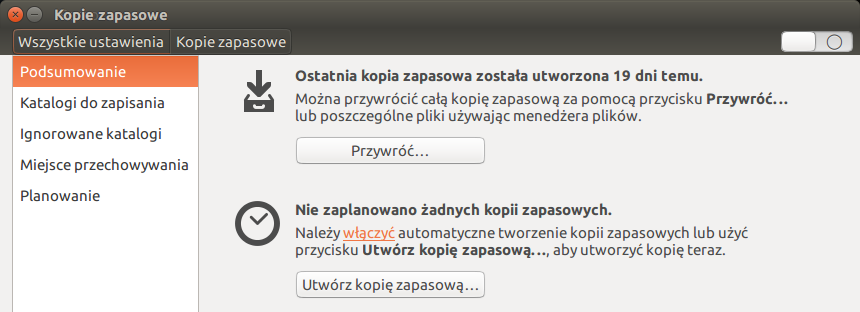
\includegraphics[width=\linewidth]{images/programy_dejavu1.png}
\end{center}

\subsubsection{Konfigurownie kopii zapasowych}
Po pierwsze należy uruchomić program Déjà Dup. Aby to zrobić wpisz w Dashu \textcolor{ubuntu_orange}{Kopie zapasowe} lub w menu systemowym 
\includegraphics{images/ikony_zasilanie.png} wybierz \menu{{Ustawienia systemu\ldots}>{Kopie Zapasowe}}.

W uruchomionym programie masz do wyboru 5 opcji. Pierwsza z nich, \textcolor{ubuntu_orange}{Podsumowanie} na razie nie jest pomocna, gdyż jeszcze nie skonfigurowałeś programu. Przejdź do \textcolor{ubuntu_orange}{Katalogi do zapisania}. Tutaj możesz wskazać, które katalogi mają być zachowywane. Domyślnie program skanuje cały katalog domowy użytkownika. Masz teraz dwie możliwości. Skasować ten wpis (przycisk \textcolor{ubuntu_orange}{-} na dolnej belce) a następnie ręcznie wskazać tylko te katalogi, które chcesz zachowywać. Dwa: pozostawić skanowanie całego katalogu domowego i wykluczyć tylko te katalogi, których na pewno nie chcesz zachowywać. Druga opcja jest lepszym rozwiązaniem, gdyż nie pominiesz niczego istotnego. łatwiej jest wykluczyć kilka katalogów niż pamiętać o włączeniu kilkuset.

Jeżeli chcesz dodać jakiś katalog naciśnij na przycisk \textcolor{ubuntu_orange}{+} i wskaż katalog spoza swojego katalogu domowego.

\textcolor{ubuntu_orange}{Ignorowane katalogi} pozwoli ci wskazać, które katalogi mają nie być zapisywane. Domyślnie pomijane są katalogi kosza oraz z plikami pobranymi z internetu {Pobrane). Warto wskazać te katalogi, o których wiadomo iż będą zajmować bardzo dużo miejsca. Filmy czy gry bardzo źle się kompresują i są bardzo duże. Nie warto ich przechowywać, chyba że cierpisz na nadmiar miejsca i mocy obliczeniowej.
\begin{itemize}
\item \textcolor{ubuntu_orange}{\textasciitilde /Filmy} --- główny katalog z filmami.
\item \textcolor{ubuntu_orange}{\textasciitilde /.wine*} --- wszystkie katalogi programu wine.
\item \textcolor{ubuntu_orange}{\textasciitilde /.local/share/Steam} --- katalog programu Steam.
\end{itemize}

\textcolor{ubuntu_orange}{Miejsce Przechowywania} wskazuje gdzie mają być zapisywane pliki z kopiami zapasowymi.  Domyślnie w katalogu domowym zostanie utworzony katalog \textcolor{ubuntu_orange}{deja-dup}, w którym będą przechowywane te pliki. Nie jest to najlepsze rozwiązanie. Podstawowa zasada tworzenia kopii zapasowych brzmi \emph{Nie należy przechowywać kopii zapasowej na tym samym nośniku co oryginalne pliki}. Alternatywne rozwiązania to:
\begin{itemize}
\item Wkazanie zamontowanego pendriva lub innego, zewnętrznego dysku.
\item Wskazanie katalogu, z którego dane są wysyłane do Chmury (nNp. DropBox, Copy).
\item Wskazanie udziału sieciowego, aby dane były przenoszone na inny komputer.
\end{itemize}

\textcolor{ubuntu_orange}{Planowanie} pozwala ustalić kiedy i z jaką częstotliwością mają być wykonywane kopie zapasowe.

Teraz możesz wrócić do zakłądki \textcolor{ubuntu_orange}{Podsumowanie}. Przycisk \textcolor{ubuntu_orange}{Utwórz kopię zapasową}. W otwartym oknie możesz wybrać, czy archiwum zostanie zaszyfrowane czy nie. Jeżeli przechowujesz kopie zapasowe na innym komputerze (np. w chmurze) to warto je zaszyfrować. Utwórz hasło i kliknij na \textcolor{ubuntu_orange}{Kontynuj}.

Aby włączyć automatyczne tworzenie kopii zapasowych upewnij się, że przełącznik w prawym górnym rogu okna jest ustawiony na pozycji \textcolor{ubuntu_orange}{Właczony},

\subsubsection{Przywracanie z backupu}
Aby przywrócić pojedyńczy plik do jego poprzedniego stanu wystarczy kliknąć na nim prawym przyciskiem myszy i wybrać \textcolor{ubuntu_orange}{Przywróć do poprzedniej wersji\ldots}. W otwartym oknie będziesz mieć możliwość wskazania, która wersja pliku ma zostać przywrócona..

Istnieje tez możliwość przywrócenia całej utworzonej kopii zapasowej. Uruchom program \textcolor{ubuntu_orange}{Kope zapasowe} i wybierz \textcolor{ubuntu_orange}{Przywróć}. Będziesz mieć możliwość wybrania, czy pliki mają zostać wypakowane do jednego katalogu, czy nadpisać aktualny stan twojego katalogu domowego. Większość zmian wprowadzonych przez drugą opcję wejdzie w życie dopiero po ponownym zalogowaniu się do systemu.